\section{OFDM Parameters}

\subsection{Primitive Parameters}

\begin{description}
	\item[BW]: This is the nominal channel bandwidth.
	\item[$N_{used}$]: Number of used subcarriers.
	\item[n]: Sampling factor. This parameter, in conjunction with BW
		and $N_{used}$ determines the subcarrier spacing, and the
		useful symbol time.
	\item[G]: This is the ratio of CP time to ``useful'' time.
\end{description}


%\todo[inline]{Insert a table of the values that are fixed by the standard and our implimentation limitations}

\subsection{Derived Parameters}

\begin{description}
	\item[$N_{FFT}$]: Smallest power of two greater than $N_{used}$
	\item[Sampling Frequency]: $F_s = floor ( n \cdot BW / 8000 )
		\times 8000 $
	\item[Subcarrier spacing]: $\Delta f = F s / N_{FFT} $
	\item[Useful symbol time]: $T_b = 1 / \Delta f$
	\item[CP Time]: $T_g = G \cdot T_b$
	\item[OFDM Symbol Time]: $T_s = T_b + T_g$
	\item[Sampling time]: $T_b / N_{FFT}$
\end{description}

% \todo[inline]{Tables of valid values for each of the derived values}

\section{External Interface to the PHY Transmitter}
\label{sec:frame}
The MAC interfaces with the PHY module by sending frames (with the
appropriate headers and padding included) as a stream of bits.  These bits
are clocked via the \textbf{mac\_clk\_in} line, and must only be sent when
the \textbf{mac\_sending\_frame} line is high.  The state of the
\textbf{mac\_sending\_frame} line must be low when not sending a frame, and
must be lowered and raised between frames that would otherwise be abutting.
The frequency of \textbf{mac\_clk\_in} must be less than or equal to half
of the \textbf{phy\_clock}.

The \textbf{phy\_ready} line is a signal to the mac that it is ready for a
new frame to be inputted, and should not be ignored.

The structure of individual frames detailed in section 8.3.5 of IEEE
802.16-2009.  Each frame contains a header, up to 4 DL sub-frames (each with
their own structure also defined in IEEE802.16-2009 section 8.3.5) and some
number of UL sub-frames.  Note that due to fixing certain implementation
parameters, some fields are constrained further than mentioned within the
standard.

\begin{description}
	\item[Frame Header - Rate\_ID] is fixed at '1' indicating CPS
		modulation with a code rate of $\frac{1}{2}$.
	
\end{description}
%\todo[inline]{Determine Full inputs and outputs}

\begin{table*} \begin{tabularx}{\linewidth}{c|c|c|X}
	\label{tbl:extern-io}
	Name & Width & Direction & Description\\ \hline

	\wire{phy\_out\_I} & 16 & O & The real component of the output,
	clocked by \wire{phy\_out\_clk} \\

	\wire{phy\_out\_Q} & 16 & O & Imaginary component of the output,
	clocked by \wire{phy\_out\_clk} \\

	\wire{phy\_out\_clk} & 1 & O & Clocks out the I and Q values
	produced by the PHY. \\

	\wire{phy\_in\_bits} & 1 & I & Input bitstream from a MAC
	device. \\

	\wire{phy\_in\_clk} & 1 & I & Clock at which the input bitstream
	\wire{phy\_in\_bits} should be sampled. \\

	\wire{phy\_in\_frame} & 1 & I & Set low while the current set of
	bits is from the same frame. Must be set high for one clock cycle
	between frames. \\

	\wire{bsid} & 4 & I & The lower four bits of the BSID, a unique
	identifier. \\
	
	\wire{bw} & 3 & I & Channel bandwidth. See \autoref{tbl:bw}. \\
\end{tabularx}
\caption{External Interface to the PHY transmitter.}
\end{table*}

\begin{table} \begin{center} \begin{tabular}{c|c}
	\label{tbl:bw}
	
	\wire{bw[3]} & Bandwidth in MHz \\ \hline

	0 & 1.25 \\
	1 & 1.5  \\
	2 & 1.75 \\
	3 & 2.0  \\
	4 & 2.75 \\
	5 - 7 & Undefined

\end{tabular} \end{center} \caption{Meanings of BW values.} \end{table}

\section{Internal Interfaces}
This section covers the interfaces for internal structures within the PHY
transmitter which are not exposed for use by the MAC or any other interfacing
hardware.

\autoref{tbl:internal-common-wire} shows some of the common signals for
the internal interfaces. \autoref{fig:flow-basic} shows the basic flow of information through the internal modules of the transmitter. Issues regarding timing, data path widths, buffering, and some minor data stream modifications are omitted.

\begin{figure}
	\begin{center}
		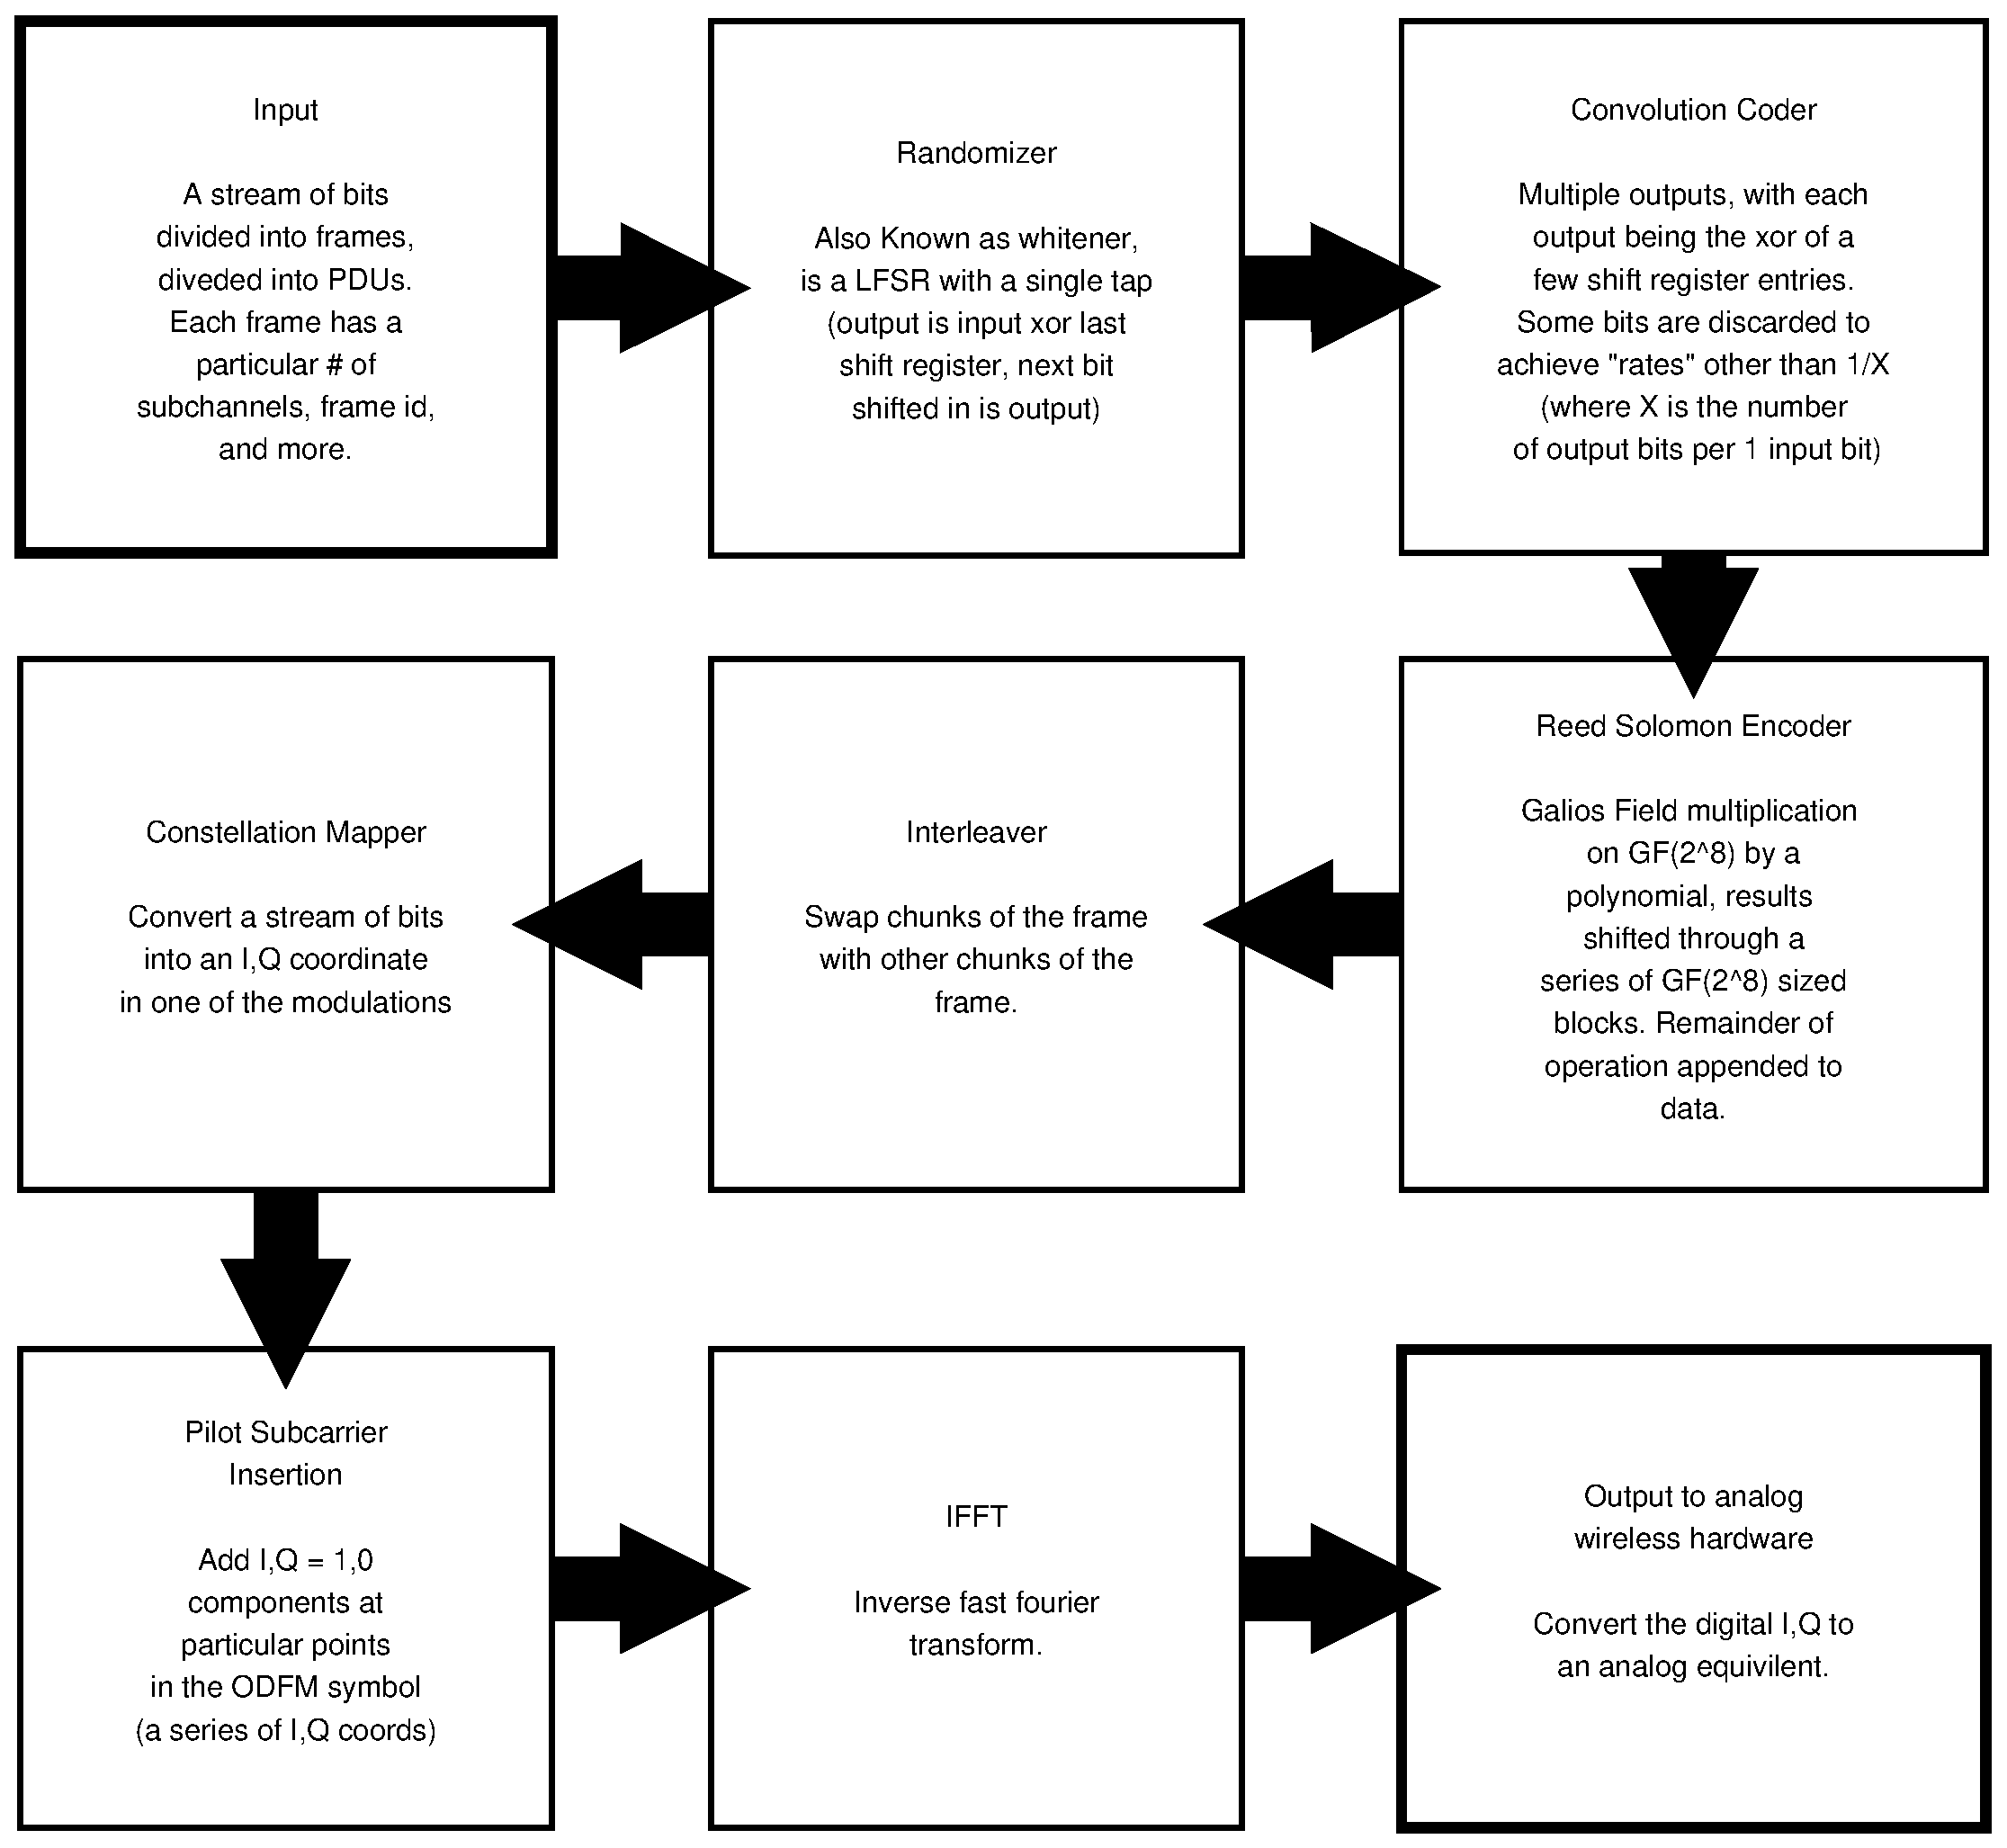
\includegraphics[width=\linewidth]{flow_basic}
		\caption{Basic flow of data through the transmitter}
		\label{fig:flow-basic}
	\end{center}
\end{figure}

\begin{table*}
\begin{tabulary}{\linewidth}{c|C|L}
	\label{tbl:internal-common-wire}
	Name & Active Level & Meaning \\ \hline
	
	\wire{*\_valid} & high & Indicate the source outputting the signal
	is also outputting data (clocked via the \wire{phy\_clock}) which
	should be processed by the next item in the chain. \\

	\wire{*\_bits} & high & A serial stream of bits clocked by
	\wire{phy\_clock}. Only valid when the corresponding
	\wire{*\_valid} line is also active. \\

	\wire{*\_flag} & high & Set active for a single clock cycle
	before becoming inactive again.
\end{tabulary}
\caption{Common signals used internally}
\end{table*}

Each block of the transmitter connected via direct wiring (without a
buffer) is given the same clock. Each block reads its inputs on alternating
clock edges such that two adjacent units read and write on different edges.
This is done so that outputted data does not change while being read.


\begin{figure}
	\begin{center}
		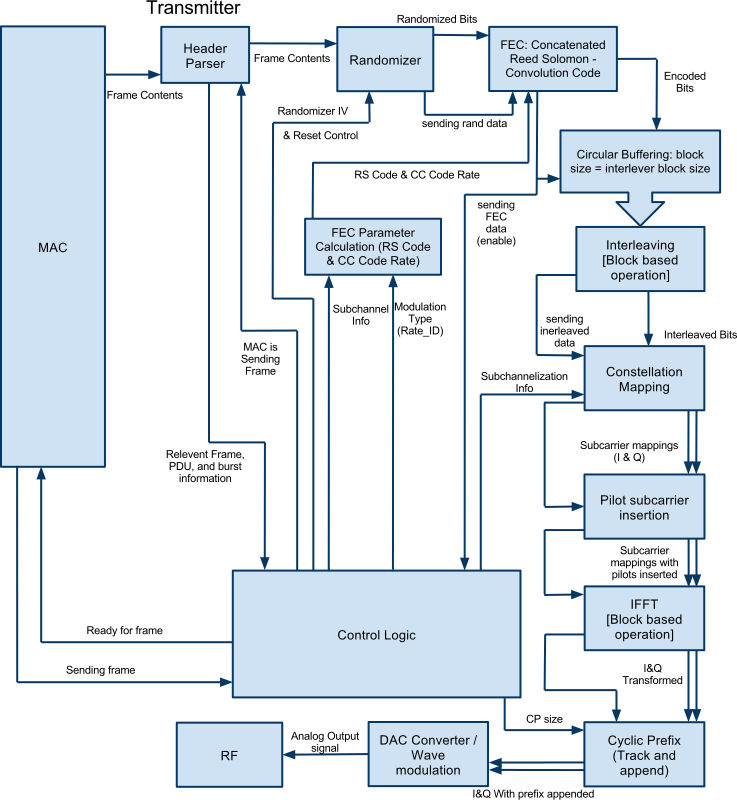
\includegraphics[width=\linewidth]{transmitter}
		\caption{More detailed diagram of the transmitter}
		\label{fig:flow-2}
	\end{center}
\end{figure}
